\clearpage
\subsection{Function} % (fold)
\label{sub:function}

Functions are used to calculate values. In many ways a Function is just like a Procedure, it has a name, can be called, can accept parameters, can have local variables, and performs a number of instructions when it is called. Unlike a Procedure, however, Functions are used to calculate values. When the function you called ends it returns back to you with a value.

\begin{figure}[h]
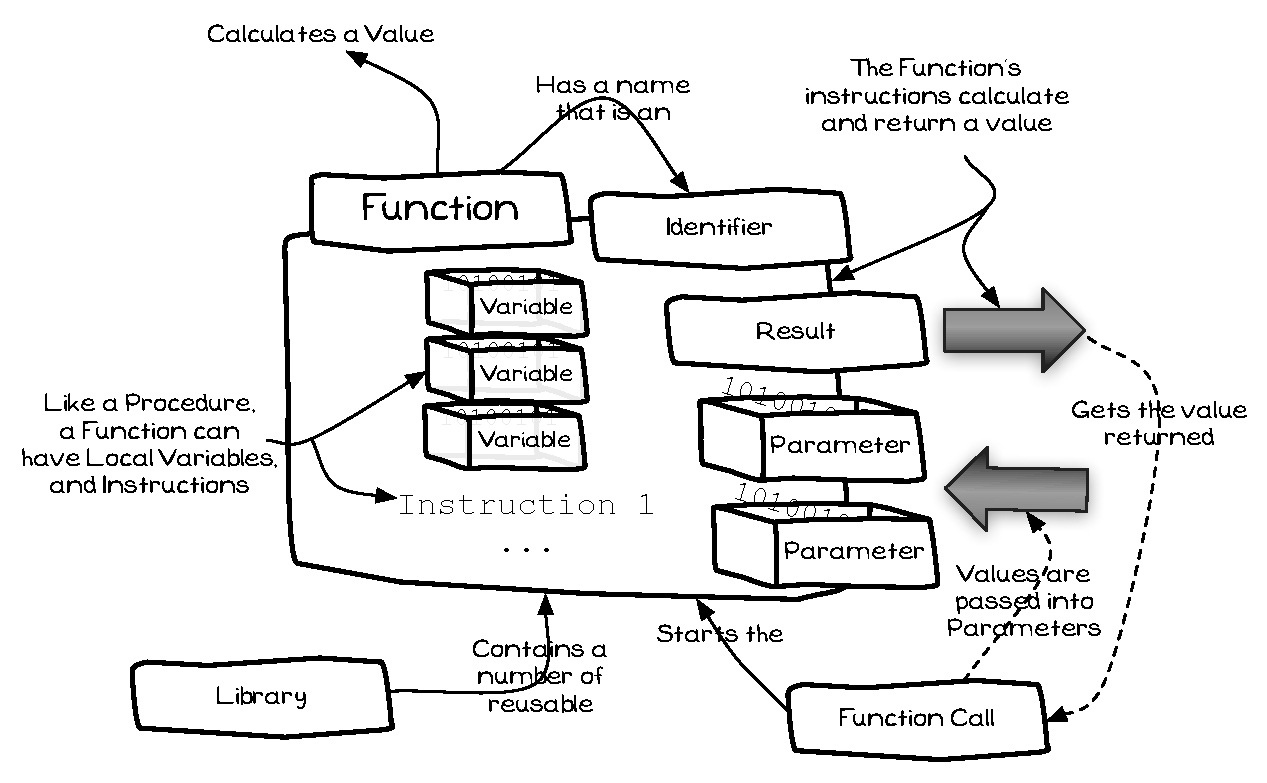
\includegraphics[width=\textwidth]{topics/storing-using-data/diagrams/Function} 
 \caption{A Function is just like a Procedure, except it calculates and returns a Value}
 \label{fig:function-decl-function}
\end{figure}

\mynote{
\begin{itemize}
  \item A Function is an \textbf{Artefact}. Something that you can create and use in your Program's code.
  \item A Function is just like a Procedure in that it ...
  \begin{itemize}
    \item Has a name that is used to call it.
    \item Performs instructions when it is executed.
    \item Can accept Parameters to allow the caller to pass in values.
    \item Is allowed to create its own local variables.
  \end{itemize}
  \item Unlike a Procedure, a Function...
  \begin{itemize}
    \item Should \textbf{not} have any side effects.
    \item Calculates and returns a value.
    \item Is called as part of an Expression.
  \end{itemize}
  \item You use Functions to calculate values.
  \item You use a \nameref{sub:function_call} to call a function as part of an Expression.
\end{itemize}
}

% subsection function (end)